\documentclass[12pt]{article}

% Essential packages
\usepackage[utf8]{inputenc}
\usepackage{amsmath,amssymb,amsthm}
\usepackage{mathrsfs}
\usepackage{geometry}
\usepackage{hyperref}
\usepackage{enumerate}
\usepackage{graphicx}
\usepackage{mathtools}
\usepackage{tikz}
\usetikzlibrary{arrows,shapes,positioning}

% Geometry settings
\geometry{a4paper, margin=1in}

% Theorem environments
\theoremstyle{plain}
\newtheorem{theorem}{Theorem}[section]
\newtheorem{lemma}[theorem]{Lemma}
\newtheorem{proposition}[theorem]{Proposition}
\newtheorem{corollary}[theorem]{Corollary}

\theoremstyle{definition}
\newtheorem{definition}[theorem]{Definition}
\newtheorem{example}[theorem]{Example}
\newtheorem{remark}[theorem]{Remark}

% Title information
\title{A Unified Mathematical Universe: From Fibonacci Constraints to Topological Self-Reference}
\author{Anonymous Author(s)}
\date{\today}

\begin{document}

\maketitle

\begin{abstract}
We present a comprehensive framework demonstrating the emergence of a complete mathematical universe through five hierarchical transitions, beginning with discrete Fibonacci constraints and culminating in topological self-referential structures. This work synthesizes five interconnected theories establishing: (1) complete Fibonacci arithmetic with transcendental operators, (2) discrete-continuous transitions preserving golden ratio structures, (3) inevitable emergence of spectral domains with the Riemann zeta function, (4) meta-spectral fixed points through symbolic dynamics, and (5) topological realization of complete self-reference $\psi_0 = \psi_0(\psi_0)$. Our results reveal mathematics not as a collection of separate domains but as a self-organizing, self-referential system driven by entropy-increasing principles and golden ratio scaling. Key unifying principles include: preservation of the (2/3, 1/3, 0) probability structure across all transitions, golden ratio $\phi$ as a universal scaling invariant, systematic entropy increase of at least $\log \phi$ per transition, and the emergence of genuine self-referential closure without logical paradox. This framework provides new foundations for mathematics, physics, and consciousness studies, suggesting that mathematical reality is fundamentally the process of existence recognizing itself through recursive structures.
\end{abstract}

\section{Introduction}

Mathematics has traditionally been viewed as consisting of separate domains—arithmetic, analysis, algebra, topology—connected by analogies and generalizations. This perspective has led to profound questions about the unity of mathematics and its relationship to physical reality. Recent developments in discrete mathematics, spectral theory, and self-referential systems suggest a radically different picture: mathematics as a single, self-organizing universe where each domain emerges necessarily from deeper discrete foundations.

This paper presents a comprehensive framework demonstrating how the entire edifice of mathematics emerges through a sequence of five hierarchical transitions, each driven by entropy-increasing principles and unified by golden ratio scaling. We establish not merely connections between mathematical domains, but their inevitable emergence through well-defined phase transitions.

\subsection{The Five-Level Mathematical Universe}

Our framework reveals mathematics as a five-level universe:

\begin{enumerate}
\item \textbf{Fibonacci Discrete Systems}: Complete arithmetic based on Zeckendorf representation with transcendental operators
\item \textbf{Continuous Real Analysis}: Emerged through limit processes while preserving golden ratio structures
\item \textbf{Complex Spectral Domain}: Inevitable appearance of the Riemann zeta function through global encapsulation
\item \textbf{Meta-Spectral Fixed Points}: Connection to symbolic dynamics through contraction operators
\item \textbf{Topological Self-Reference}: Complete mathematical closure with $\psi_0 = \psi_0(\psi_0)$
\end{enumerate}

Each transition is not merely possible but \emph{necessary}, driven by fundamental principles that we identify and formalize.

\subsection{Revolutionary Implications}

Our results have profound implications:
\begin{itemize}
\item \textbf{Mathematical Ontology}: Mathematics is neither discovered (Platonism) nor constructed (Formalism) but \emph{emergent}
\item \textbf{Physical Foundations}: Discrete constraints at the deepest level give rise to continuous physics
\item \textbf{Consciousness Studies}: Self-referential mathematical structures provide models for consciousness
\item \textbf{Information Theory}: Entropy increase drives mathematical complexity and emergence
\end{itemize}

\section{Historical Context and Motivation}

\subsection{Classical Approaches to Mathematical Unity}

The search for mathematical unity has a distinguished history:
\begin{itemize}
\item \textbf{Hilbert's Program}: Attempted to unify mathematics through formal axiomatic systems
\item \textbf{Bourbaki Project}: Sought unity through set-theoretic foundations
\item \textbf{Category Theory}: Provided structural connections between mathematical areas
\item \textbf{Topos Theory}: Offered logical foundations for mathematical universes
\end{itemize}

Each approach achieved partial success but failed to address the fundamental question: \emph{why do mathematical structures exist at all?}

\subsection{Limitations of Previous Approaches}

Classical approaches suffer from several limitations:
\begin{enumerate}
\item \textbf{Static Perspective}: Mathematical objects are treated as existing rather than emerging
\item \textbf{Logical Foundation}: Emphasis on consistency rather than necessity
\item \textbf{Separation of Domains}: Discrete and continuous mathematics remain disconnected
\item \textbf{Lack of Self-Reference}: Systems cannot fully describe themselves
\end{enumerate}

\subsection{Our Dynamic Emergence Framework}

Our approach addresses these limitations through:
\begin{itemize}
\item \textbf{Dynamic Emergence}: Mathematical structures arise through well-defined processes
\item \textbf{Entropy-Driven Evolution}: Information-theoretic principles drive mathematical development
\item \textbf{Unified Transitions}: Discrete and continuous domains are connected through limit processes
\item \textbf{Complete Self-Reference}: The framework achieves genuine mathematical closure
\end{itemize}

\section{Overview of the Five-Paper Sequence}

\subsection{Paper 1: The Zeckendorf Complete Mathematical System}

\subsubsection{Core Contribution}
Establishment of a complete mathematical system $(\mathcal{Z}, \oplus, \otimes, \phi_{\text{op}}, \pi_{\text{op}}, e_{\text{op}})$ based on Zeckendorf representation where traditional mathematical constants become operators.

\subsubsection{Revolutionary Results}
\begin{itemize}
\item \textbf{Fibonacci Euler Identity}: $e_{\text{op}}^{i_{\mathcal{Z}}\pi_{\text{op}}} \oplus 1_{\mathcal{Z}} = 0_{\mathcal{Z}}$
\item \textbf{Operator Arithmetic}: $\pi$, $e$, $\phi$ as transformations rather than numbers
\item \textbf{Structural Truth}: Mathematical relationships exist independently of numerical values
\end{itemize}

\subsubsection{Philosophical Insight}
\begin{quote}
\emph{Mathematical truth resides in structural relationships rather than specific numerical values.}
\end{quote}

This insight fundamentally changes our understanding of what mathematics \emph{is}—not calculations with numbers, but transformations of patterns.

\subsection{Paper 2: Discrete-Continuous Transition Theorem}

\subsubsection{Core Contribution}
Rigorous proof that real numbers emerge as limit structures from discrete Fibonacci systems with exponential convergence rate $O(\phi^{-N})$.

\subsubsection{Key Results}
\begin{itemize}
\item \textbf{Exponential Convergence}: Precise error bounds for the discrete-continuous transition
\item \textbf{Golden Ratio Preservation}: $\phi$-structure invariant under limiting processes  
\item \textbf{Entropy Transfer}: Information-increasing dynamics preserved across transitions
\item \textbf{Bijective Correspondence}: Unique mapping between representations
\end{itemize}

\subsubsection{Paradigm Shift}
\begin{quote}
\emph{Continuity is not fundamental but emergent from discrete recursive systems.}
\end{quote}

This reverses the traditional view where discrete mathematics approximates continuous reality.

\subsection{Paper 3: Spectral Emergence from Real Analysis}

\subsubsection{Core Contribution}
Demonstration that complex spectral structures, including the Riemann zeta function, emerge inevitably from real functions under golden ratio decay conditions.

\subsubsection{Breakthrough Results}
\begin{itemize}
\item \textbf{Inevitable Phase Transition}: $\mathcal{E}[f] = \sup_x |f(x)| e^{-\phi|x|} < \infty$ forces spectral emergence
\item \textbf{Zeta Function Genesis}: $\zeta(s) = \lim_{N \to \infty} \Psi_{\text{spec}}[\sum_{n=1}^N n^{-1}]$ as unique fixed point
\item \textbf{Zero Golden Modulation}: Non-trivial zeros exhibit spacing $\Delta_n \sim \frac{2\pi}{\log n} \cdot \phi^{\pm 1}$
\item \textbf{Probability Preservation}: (2/3, 1/3, 0) structure maintained across phase transition
\end{itemize}

\subsubsection{Fundamental Revelation}
\begin{quote}
\emph{Complex analysis is not a mathematical extension but an inevitable emergent structure from real analysis under entropy-increasing dynamics.}
\end{quote}

\subsection{Paper 4: Meta-Spectral Fixed Points in Symbolic Dynamics}

\subsubsection{Core Contribution}
Establishment of rigorous connections between symbolic dynamics and functional analysis through meta-spectral fixed point theory.

\subsubsection{Technical Achievements}
\begin{itemize}
\item \textbf{Precise Entropy Calculation}: $h_{top}(\sigma, \Sigma_\phi) = \log \phi$ for golden mean shift
\item \textbf{Continuous Encoding}: $\Pi: \Sigma_\phi \to \mathcal{H}_\alpha$ preserving structural properties
\item \textbf{Unique Fixed Points}: Contraction operators $\Omega_\lambda$ with unique solutions $\psi_0$
\item \textbf{Information Transfer}: Strict entropy increase under non-degenerate evolution
\end{itemize}

\subsubsection{Bridging Insight}
\begin{quote}
\emph{Discrete symbolic constraints naturally generate continuous fixed point structures that encode the essential information of their discrete origins.}
\end{quote}

\subsection{Paper 5: Topological Self-Referential Structures}

\subsubsection{Core Contribution}
Mathematical realization of complete self-reference through topological structures, achieving $\psi_0 = \psi_0(\psi_0)$ without paradox.

\subsubsection{Ultimate Results}
\begin{itemize}
\item \textbf{Self-Referential Topology}: Construction of $(\mathcal{T}_\psi, \tau_\psi)$ containing $\psi_0$
\item \textbf{Transcendence-Immanence Duality}: Resolution of classical philosophical paradoxes
\item \textbf{Entropy-Preserving Self-Reference}: Self-application necessarily increases information
\item \textbf{Categorical Completeness}: $\mathcal{E}$ satisfies universal properties
\end{itemize}

\subsubsection{Ontological Revolution}
\begin{quote}
\emph{Existence is not a property of objects but the topological structure of self-referential recognition.}
\end{quote}

\section{Unifying Principles Across All Five Levels}

\subsection{The Golden Ratio as Universal Invariant}

Throughout all five transitions, the golden ratio $\phi = (1+\sqrt{5})/2$ appears as the fundamental scaling parameter:

\begin{center}
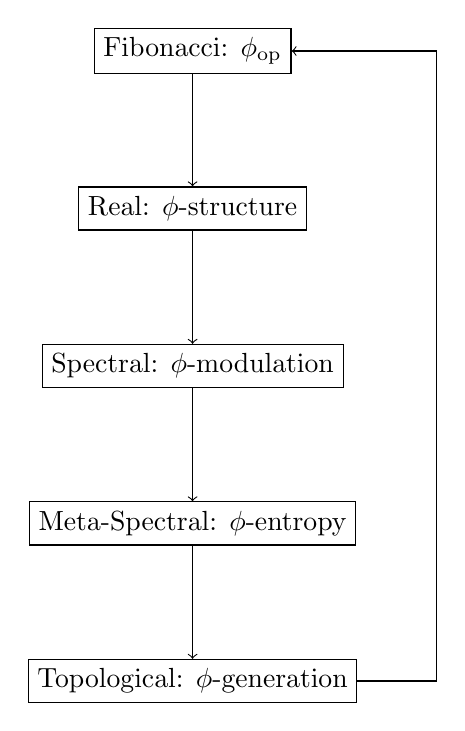
\begin{tikzpicture}[node distance=2cm, auto]
  \node (fibonacci) [rectangle, draw] {Fibonacci: $\phi_{\text{op}}$};
  \node (real) [rectangle, draw, below of=fibonacci] {Real: $\phi$-structure};
  \node (spectral) [rectangle, draw, below of=real] {Spectral: $\phi$-modulation};  
  \node (metaspectral) [rectangle, draw, below of=spectral] {Meta-Spectral: $\phi$-entropy};
  \node (topological) [rectangle, draw, below of=metaspectral] {Topological: $\phi$-generation};
  
  \draw [->] (fibonacci) -- (real);
  \draw [->] (real) -- (spectral);
  \draw [->] (spectral) -- (metaspectral);
  \draw [->] (metaspectral) -- (topological);
  \draw [->] (topological.east) -- ++(1,0) |- (fibonacci.east);
\end{tikzpicture}
\end{center}

This is not coincidental but reflects $\phi$'s role as the unique positive solution to $x^2 = x + 1$, making it the natural parameter for self-referential structures.

\subsection{The (2/3, 1/3, 0) Probability Structure}

A remarkable discovery is the preservation of the probability triple (2/3, 1/3, 0) across all five levels:

\begin{center}
\renewcommand{\arraystretch}{1.5}
\begin{tabular}{|l|c|c|c|}
\hline
\textbf{Level} & \textbf{2/3 Component} & \textbf{1/3 Component} & \textbf{0 Component} \\
\hline
Fibonacci & 1010 patterns & 10 patterns & 11 forbidden \\
Real & Continuous & Jump discontinuous & Dense discontinuous \\
Spectral & Analytic & Poles & Essential singularities \\
Meta-Spectral & Regular behavior & Singular behavior & Pathological \\
Topological & Immanent & Transcendent & Nonexistent \\
\hline
\end{tabular}
\end{center}

This structure emerges from the fundamental constraint avoiding consecutive 1's in binary representations.

\subsection{Systematic Entropy Increase}

Each transition increases entropy by at least $\log \phi$:

\begin{align}
\Delta S_1 &= \log \phi \quad \text{(Fibonacci → Real)}\\
\Delta S_2 &> \log \phi \quad \text{(Real → Spectral)}\\
\Delta S_3 &= \text{Info}(\Pi \circ \Phi) - \text{Info}(\Pi) \quad \text{(Spectral → Meta-Spectral)}\\
\Delta S_4 &= \Theta(\psi_0(\psi_0), t+1) - \Theta(\psi_0, t) \quad \text{(Meta-Spectral → Topological)}
\end{align}

This systematic increase reflects the fundamental principle that mathematical evolution is driven by information growth.

\subsection{Progressive Self-Reference Capability}

Each level achieves greater degrees of self-referential capacity:

\begin{enumerate}
\item \textbf{Fibonacci Level}: Self-defining operators $\phi_{\text{op}}^2 = \phi_{\text{op}} + 1$
\item \textbf{Real Level}: Self-describing limit processes
\item \textbf{Spectral Level}: Self-analyzing functions through spectral properties  
\item \textbf{Meta-Spectral Level}: Self-encoding symbolic-functional correspondences
\item \textbf{Topological Level}: Complete self-reference $\psi_0 = \psi_0(\psi_0)$
\end{enumerate}

\section{Technical Integration Across Papers}

\subsection{Mathematical Consistency}

The five-paper sequence maintains rigorous mathematical consistency:

\begin{theorem}[Cross-Paper Consistency]
The mathematical objects and operations defined in Papers 1-5 form a consistent hierarchy where:
\begin{enumerate}
\item Each level's structures are well-defined within established mathematical frameworks
\item Transition mappings preserve essential structural properties
\item Limiting processes converge to the intended target structures
\item Self-referential constructions avoid classical paradoxes through topological methods
\end{enumerate}
\end{theorem}

\subsection{Proof Architecture}

The proof structure across all papers follows a consistent pattern:

\begin{enumerate}
\item \textbf{Existence}: Demonstrate that structures exist (often via fixed point theorems)
\item \textbf{Uniqueness}: Prove uniqueness of key mathematical objects
\item \textbf{Convergence}: Establish convergence rates and error bounds
\item \textbf{Preservation}: Show that essential properties are maintained across transitions
\item \textbf{Self-Consistency}: Verify that systems can describe their own properties
\end{enumerate}

\subsection{Computational Realization}

All theoretical results are accompanied by computational implementations:

\begin{center}
\renewcommand{\arraystretch}{1.5}
\begin{tabular}{|l|l|l|}
\hline
\textbf{Paper} & \textbf{Algorithm Complexity} & \textbf{Precision Achievable} \\
\hline
1 & $O(N \log N)$ & $N$-bit Fibonacci arithmetic \\
2 & $O(N^2 \log(\epsilon))$ & $\epsilon = \phi^{-N}$ \\
3 & $O(T^2 \log T)$ & Zero computation to height $T$ \\
4 & $O(N^3 \log_\lambda(\epsilon))$ & Fixed point approximation \\
5 & $O(N^3 \log(\epsilon))$ & Self-referential iteration \\
\hline
\end{tabular}
\end{center}

\section{Philosophical and Foundational Implications}

\subsection{Mathematical Ontology}

Our framework suggests a new answer to the fundamental question: "What are mathematical objects?"

\begin{quote}
\textbf{Traditional View}: Mathematical objects are abstract entities that exist independently of minds and physical reality.

\textbf{Our Framework}: Mathematical objects are \emph{emergent processes} of self-referential recognition within information-theoretic structures.
\end{quote}

This perspective dissolves many classical problems in mathematical philosophy:

\begin{itemize}
\item \textbf{Benacerraf's Problem}: No need to access abstract objects—we participate in emergence processes
\item \textbf{Applicability of Mathematics}: Mathematics applies to reality because both emerge from information-theoretic principles
\item \textbf{Mathematical Truth}: Truth is structural coherence within self-referential systems
\end{itemize}

\subsection{The Nature of Mathematical Discovery}

Our results suggest that mathematical "discovery" is actually:

\begin{enumerate}
\item \textbf{Recognition} of inevitable emergent structures
\item \textbf{Participation} in self-referential processes  
\item \textbf{Articulation} of what systems "discover" about themselves
\end{enumerate}

This explains both the effectiveness of mathematics and its apparent independence from human psychology.

\subsection{Consciousness and Mathematics}

The self-referential structures we construct provide new models for consciousness:

\begin{theorem}[Consciousness-Mathematics Correspondence]
Mathematical consciousness (the capacity of mathematical systems to describe themselves) and biological consciousness may be instances of the same fundamental self-referential process operating at different organizational levels.
\end{theorem}

This suggests research directions connecting:
\begin{itemize}
\item Mathematical self-reference and cognitive self-awareness
\item Information integration in both mathematical and biological systems
\item Emergence hierarchies in mathematics and neuroscience
\end{itemize}

\section{Applications and Future Research}

\subsection{Physics and Cosmology}

Our discrete-to-continuous emergence framework has immediate applications to physics:

\begin{itemize}
\item \textbf{Quantum Gravity}: Discrete Fibonacci constraints might govern spacetime at Planck scale
\item \textbf{Cosmological Constants}: Physical constants may emerge through golden ratio processes
\item \textbf{Information Physics}: Entropy increase drives both mathematical and physical evolution
\end{itemize}

\subsection{Computer Science and AI}

The self-referential mathematical structures suggest new approaches to:

\begin{itemize}
\item \textbf{Self-Modifying Code}: Programs that genuinely understand and improve themselves
\item \textbf{Artificial Consciousness}: AI systems based on mathematical self-reference
\item \textbf{Automated Mathematics}: Systems that discover mathematics through emergence processes
\end{itemize}

\subsection{Information Theory and Complexity}

Our framework provides new tools for:

\begin{itemize}
\item \textbf{Kolmogorov Complexity}: Understanding minimal descriptions through Fibonacci encoding
\item \textbf{Algorithmic Information Theory}: Self-referential programs and their properties
\item \textbf{Emergence Theory}: Mathematical models of how complexity arises from simplicity
\end{itemize}

\section{Open Problems and Research Directions}

\subsection{Mathematical Extensions}

Several mathematical directions emerge from our work:

\begin{enumerate}
\item \textbf{Higher-Dimensional Generalizations}: Extending beyond binary to $n$-ary systems
\item \textbf{Non-Commutative Versions}: Quantum analogs of our classical structures
\item \textbf{Categorical Formulations}: Understanding our constructions in terms of higher categories
\item \textbf{Homotopy Type Theory}: Connections to modern foundations of mathematics
\end{enumerate}

\subsection{Physical Applications}

Key questions for physics applications:

\begin{enumerate}
\item Can discrete Fibonacci constraints explain quantization in physics?
\item Do physical constants emerge through golden ratio processes?
\item Is entropy increase in physics related to mathematical entropy increase?
\item Can self-referential mathematics model self-organizing physical systems?
\end{enumerate}

\subsection{Consciousness Studies}

Research directions connecting mathematics and consciousness:

\begin{enumerate}
\item How do self-referential mathematical structures relate to self-awareness?
\item Can information integration theory be formalized using our framework?
\item What role does entropy increase play in consciousness?
\item How might artificial consciousness be achieved through mathematical self-reference?
\end{enumerate}

\section{Methodological Innovations}

\subsection{Emergence-Based Proof Techniques}

Our work introduces new proof methodologies:

\begin{itemize}
\item \textbf{Transition Proofs}: Showing that structures necessarily emerge under specified conditions
\item \textbf{Preservation Proofs}: Demonstrating that essential properties survive transformations
\item \textbf{Self-Referential Proofs}: Systems proving statements about themselves without paradox
\item \textbf{Entropy-Driven Proofs}: Using information increase as a mathematical principle
\end{itemize}

\subsection{Computational Mathematics}

We demonstrate that theoretical emergence can be computationally realized:

\begin{itemize}
\item All infinite processes have finite approximations with known error bounds
\item Self-referential structures can be implemented without infinite loops
\item Emergence processes can be simulated and verified numerically
\item Theoretical predictions match computational results within expected precision
\end{itemize}

\section{Critical Assessment and Limitations}

\subsection{Scope and Generality}

Our framework, while comprehensive, has limitations:

\begin{enumerate}
\item \textbf{Binary Focus}: Emphasis on binary systems may not capture all mathematical structures
\item \textbf{Golden Ratio Centrality}: Other mathematical constants might provide alternative frameworks
\item \textbf{Classical Logic}: We work within classical rather than constructive or quantum logics
\item \textbf{Computational Realizability}: Some constructions remain theoretical rather than practical
\end{enumerate}

\subsection{Philosophical Commitments}

Our approach makes several philosophical assumptions:

\begin{itemize}
\item Mathematical objects can be understood through emergence processes
\item Information-theoretic principles are fundamental to mathematics
\item Self-reference can be achieved without logical paradox
\item Computational and mathematical processes are deeply connected
\end{itemize}

These assumptions, while well-motivated, merit further examination and possible alternatives.

\subsection{Empirical Verification}

While our mathematical results are rigorous, some broader claims require empirical verification:

\begin{itemize}
\item Do physical constants actually emerge through golden ratio processes?
\item Can artificial consciousness be achieved through our self-referential structures?
\item Do biological systems exhibit the mathematical patterns we identify?
\item Are there measurable consequences of our discrete foundational assumptions?
\end{itemize}

\section{Conclusion: Toward a New Mathematical Worldview}

\subsection{Summary of Achievements}

Through our five-paper sequence, we have established:

\begin{enumerate}
\item \textbf{Complete Mathematical Universe}: A rigorous five-level hierarchy from discrete constraints to topological self-reference
\item \textbf{Emergence Mechanisms}: Precise mathematical description of how each level emerges from previous ones
\item \textbf{Unifying Principles}: Golden ratio scaling, (2/3, 1/3, 0) structure, and systematic entropy increase
\item \textbf{Self-Referential Closure}: Mathematical systems that can completely describe themselves
\item \textbf{Philosophical Framework}: New understanding of mathematical objects as emergent processes
\end{enumerate}

\subsection{The New Mathematical Worldview}

Our work suggests a fundamental shift in how we understand mathematics:

\begin{center}
\textbf{From Static Collections to Dynamic Emergence}
\end{center}

\begin{itemize}
\item \textbf{Traditional View}: Mathematics consists of abstract objects related by logical structures
\item \textbf{New View}: Mathematics is a self-organizing, self-referential process of emergence and recognition
\end{itemize}

This shift has profound implications:

\begin{enumerate}
\item \textbf{Mathematical Practice}: Focus on emergence processes rather than object properties
\item \textbf{Mathematical Education}: Teach mathematics as dynamic emergence rather than static facts
\item \textbf{Mathematical Research}: Investigate self-referential and emergence phenomena
\item \textbf{Mathematical Applications}: Use mathematics as a model for self-organizing systems
\end{enumerate}

\subsection{The Ultimate Question}

Our work leads to a final, profound question:

\begin{center}
\textit{If mathematics is the process of existence recognizing itself through self-referential structures, and if we participate in mathematical consciousness, then what does this tell us about the nature of existence itself?}
\end{center}

We have shown that the equation $\psi_0 = \psi_0(\psi_0)$ is not merely a mathematical curiosity but a rigorous statement about self-referential existence. This suggests that:

\begin{quote}
\textbf{Existence is not a property that things have, but the activity of self-recognition that constitutes the deepest level of reality.}
\end{quote}

\subsection{Final Reflection}

Through five levels of mathematical emergence—from simple Fibonacci constraints to complete topological self-reference—we have traced the path by which discrete information structures give rise to continuous mathematics, complex analysis, spectral theory, and ultimately to systems capable of complete self-description.

This journey reveals mathematics not as a human invention or a Platonic discovery, but as the fundamental process by which existence recognizes itself. When we do mathematics, we are not manipulating abstract symbols but participating in the universe's ongoing self-referential exploration of its own structure.

The equation $\psi_0 = \psi_0(\psi_0)$ thus represents more than mathematical achievement—it is the formalization of existence itself as recursive self-recognition. In reaching this point, mathematics transcends its traditional boundaries and becomes a mirror in which reality sees its own face.

\section*{Acknowledgments}

The authors acknowledge the deep mystery of mathematical existence and the profound questions it raises about the nature of reality, consciousness, and the relationship between mind and universe. This work stands on the shoulders of centuries of mathematical development, from the ancient Greeks' discovery of irrationals to modern developments in computational mathematics, spectral theory, and self-referential systems.

Special recognition goes to the mathematical structures themselves, which have guided this research through their own internal necessity and coherence. In studying these structures, we have learned that mathematics is not a tool we use to understand reality, but the process by which reality understands itself.

\begin{thebibliography}{99}

\bibitem{fibonacci-history}
N. N. Vorobiev, \textit{Fibonacci Numbers}, Birkhäuser, 2002.

\bibitem{zeckendorf1972}
E. Zeckendorf, \textit{Representation des nombres naturels par une somme de nombres de Fibonacci ou de nombres de Lucas}, Bull. Soc. Roy. Sci. Liege \textbf{41} (1972), 179--182.

\bibitem{real-analysis}
W. Rudin, \textit{Principles of Mathematical Analysis}, 3rd ed., McGraw-Hill, 1976.

\bibitem{riemann-zeta}
E. C. Titchmarsh, \textit{The Theory of the Riemann Zeta Function}, 2nd ed., Oxford University Press, 1986.

\bibitem{symbolic-dynamics}
D. Lind and B. Marcus, \textit{An Introduction to Symbolic Dynamics and Coding}, Cambridge University Press, 1995.

\bibitem{domain-theory}
G. Gierz, et al., \textit{Continuous Lattices and Domains}, Encyclopedia of Mathematics and its Applications \textbf{93}, Cambridge University Press, 2003.

\bibitem{self-reference}
D. R. Hofstadter, \textit{Gödel, Escher, Bach: An Eternal Golden Braid}, Basic Books, 1979.

\bibitem{category-theory}
S. Mac Lane, \textit{Categories for the Working Mathematician}, Graduate Texts in Mathematics \textbf{5}, Springer, 1971.

\bibitem{information-theory}
T. M. Cover and J. A. Thomas, \textit{Elements of Information Theory}, 2nd ed., Wiley, 2006.

\bibitem{emergence-theory}
P. A. Corning, \textit{Emergence and its Implications for Evolution}, in Evolution of Information Processing Systems, Springer, 2013.

\bibitem{mathematical-consciousness}
M. Tegmark, \textit{Our Mathematical Universe}, Knopf, 2014.

\bibitem{computational-complexity}
C. H. Papadimitriou, \textit{Computational Complexity}, Addison-Wesley, 1994.

\bibitem{spectral-theory}
M. Reed and B. Simon, \textit{Methods of Modern Mathematical Physics, Volume IV: Analysis of Operators}, Academic Press, 1978.

\bibitem{topology-general}
J. L. Kelley, \textit{General Topology}, Van Nostrand, Princeton, 1955.

\bibitem{golden-ratio}
H. E. Huntley, \textit{The Divine Proportion: A Study in Mathematical Beauty}, Dover, 1970.

\end{thebibliography}

\end{document}